\begin{chapabstract}
\small{
This chapter presents the results of the p-value analyses and performance benchmarks. \autoref{s:Experiment-Setup} reintroduces the scientific use cases and the assumptions made in these scenarios. It then describes the test set generation process. \autoref{s:p-values-results} presents the results of the p-value analysis. \autoref{s:architectures-comparison} shows a comparison between the two investigated autoencoder architectures. \autoref{s:ad-vs-lima} outlines the performances of the proposed anomaly detection method against the Li\&Ma standard technique. The key performance indicators used for the comparison are introduced. The results for both use cases of serendipitous discoveries and follow-up observations are presented in the short-exposure and very short-exposure scenarios.
}\\
\begin{center}
\noindent\makebox[0.8\linewidth]{\rule{0.66\paperwidth}{0.4pt}}
\end{center}
\vspace{1cm}
\end{chapabstract}

\section{Experiments setup}
\label{s:Experiment-Setup}
This chapter presents the results of a study aimed to develop an anomaly detection technique for addressing the real-time source detection problem in the context of the Cherenkov Telescope Array Observatory (CTAO). As outlined in \autoref{s:contribution}, the proposed anomaly detection technique is based on an autoencoder model. Two autoencoder architectures based on convolutional and recurrent layers have been investigated. The comparison of their performances evaluated with standard machine learning metrics will be presented in this chapter. A p-value statistical analysis was performed to determine the classification thresholds the models can use to associate $5\sigma$ statistical significances to positive detections. This chapter will also present the results of these analyses. 
This chapter focuses on verifying if the proposed technique overcomes the limitations of the standard analyses presented in \autoref{ss:li-ma} and \autoref{ss:ffov-ml} obtains better performances in practice. Key performance indicators (KPIs) have been defined in the context of two scientific use cases: \textit{serendipitous discovery} and \textit{follow-up observations}, introduced in \autoref{s:contribution-1-use-cases}. The results have been compared against the performances of the Li\&Ma analysis technique. The KPIs were first evaluated in the short-exposure scenario, using an integration time of 5 seconds meaning that each point of the sub-sequences aggregates 5 seconds of data. Furthermore, the same evaluations were repeated in the very short-exposure scenario, using an integration time of 1 second. The next section will re-introduce the scientific use cases of serendipitous discovery and follow-up observations, highlighting the assumptions and the experiments' setup.

\subsection{Scientific use cases and assumptions}
\label{ss:scientific-use-cases-and-assumptions}
The serendipitous discoveries use case models the scenario in which the telescopes are observing a certain sky region, and an unexpected event is seen in the field of view. This kind of discovery is possible even though the probability of a serendipitous GRB event appearing in the field of view during an observation is very low. Indeed, telescopes can systematically observe large sky regions, for example, during surveys, increasing the probability of serendipitous discoveries. Such events are scientifically crucial because the overall evolution of the GRB event can be observed from the beginning. To maximize the scientific return, detecting the serendipitous source should be addressed as soon as possible to let other observatories acknowledge the discovery through a science alert broadcasted to the scientific community. By doing so, the same events can be studied with other instruments, exploring different wavelengths or messengers. 
As explained in \autoref{ss:aperture-photometry}, the aperture photometry method defines an aperture, a closed region centered on the source, to count the on-source photons. The issue is that we don't know in which region the GRB event will appear. One way to address the problem is to use several regions as shown by \autoref{fig:rings}. The problem with this approach is the significant increase in the number of analysis trials, which must be considered as a post-trials probability. In the context of this work, another assumption is made, a blind-search analysis applied in the whole field of view in order to localize candidate sources in the least possible amount of time. One example of blind-search implementation is provided by CTools \cite{Knodlseder_2016}, executing a peak-detection algorithm on smoothed count maps with a localization acceptance threshold above a given significance. It is assumed that the blind-search analysis will always find the region that contains the GRB event in its center for each GRB event considered in the performance analysis. It is also assumed that blind-search will always take a fixed time of 10 seconds to find the region. 

The observatory must not only be the sender of scientific alerts but also be capable of receiving and reacting to external ones. The follow-up observation use case models the scenario in which the observatory receives a science alert and changes the pointing of its telescope to a new sky region to detect the event. Several considerations should be made. The time that passes from the event's start and the taking of the first photon counts, is variable. It depends on two factors: the time to receive the scientific alert and the time the telescopes take to change the pointing. This delay has been considered with four different values: 25, 50, 75, and 100 seconds. After this delay, once the required data is obtained, the analysis techniques can start to perform classifications. Unlike the serendipitous discovery scenario, the evolution of the GRB event cannot be observed from the beginning. The luminosity of a GRB event tends to decrease over time, increasing the difficulty of detection. Another factor to consider is the localization error on the position of the source provided by the received scientific alert. This error can be smaller than the field of view or much larger, as in the case of a gravitational-wave alert. The latter case would require multiple observations performed with a tiling strategy \cite{seglar2019gravitational}, but this is outside of the scope of this work. If the localization error within the field of view must be covered by multiple aperture photometry regions, the blind-search approach used in the serendipitous scenario will also be considered here.   

 
\subsection{Test set generation}
\label{s:Experiment-Data}
The test set used for the performance evaluation of the proposed anomaly detection method is a supervised data set containing two classes of samples. The first class of samples has been generated considering the background model in the simulations. The second class of samples has been generated considering the background and source models in the simulations. The templates used for the Gamma-Ray Bursts (GRBs) simulations were taken from the POSyTIVE catalog. The mock GRB population used by POSyTIVE is calibrated using a 40-year data set of multi-wavelength GRB observations \cite{Bernardini_2019}, providing about 20 thousand GRB templates of known events.
As stated in \autoref{s:Gamma-Ray-Bursts}, GRBs are characterized by several key properties, including duration and peak flux. The latter measures the maximum energy level emitted by the event. It is usually measured in units of $erg/s/cm^2$ and is one of the most important parameters for characterizing the luminosity of a GRB. GRBs can have a wide range of peak fluxes, from as low as $10^-9 erg/s/cm^2$ to as high as $10^-5 erg/s/cm^2$, depending on the distance and its intrinsic properties. If the luminosity is too low, the GRB event will be indistinguishable from the background noise. For this reason, but also computational resource limitations, only a subset of the entire catalog has been simulated. 
The mean of the background level has been considered a threshold to limit the number of simulations. The test set has been generated simulating all the templates whose peak flux is greater or equal to the background level mean minus $1\sigma$, to account for the background fluctuations. Figure~\ref{f:exp-max-flux-distribution-E} shows the distribution of the peak flux of each GRB template and highlights the selected set. As explained in \autoref{ss:dl3-simulator}, the simulation tool generates a photons list, i.e., a list of photons whose energy and arrival direction are reconstructed. Only the GRB afterglow model has been simulated since the prompt models were not available at the time of writing. The simulation tool has been used to generate one simulated trial for each selected template. The resulting test set contains 419 trials with a peak flux in the interval $[2.6785e^{-10}, 1.1688e^{-04}]$.
\begin{figure}[!htb]
\centering
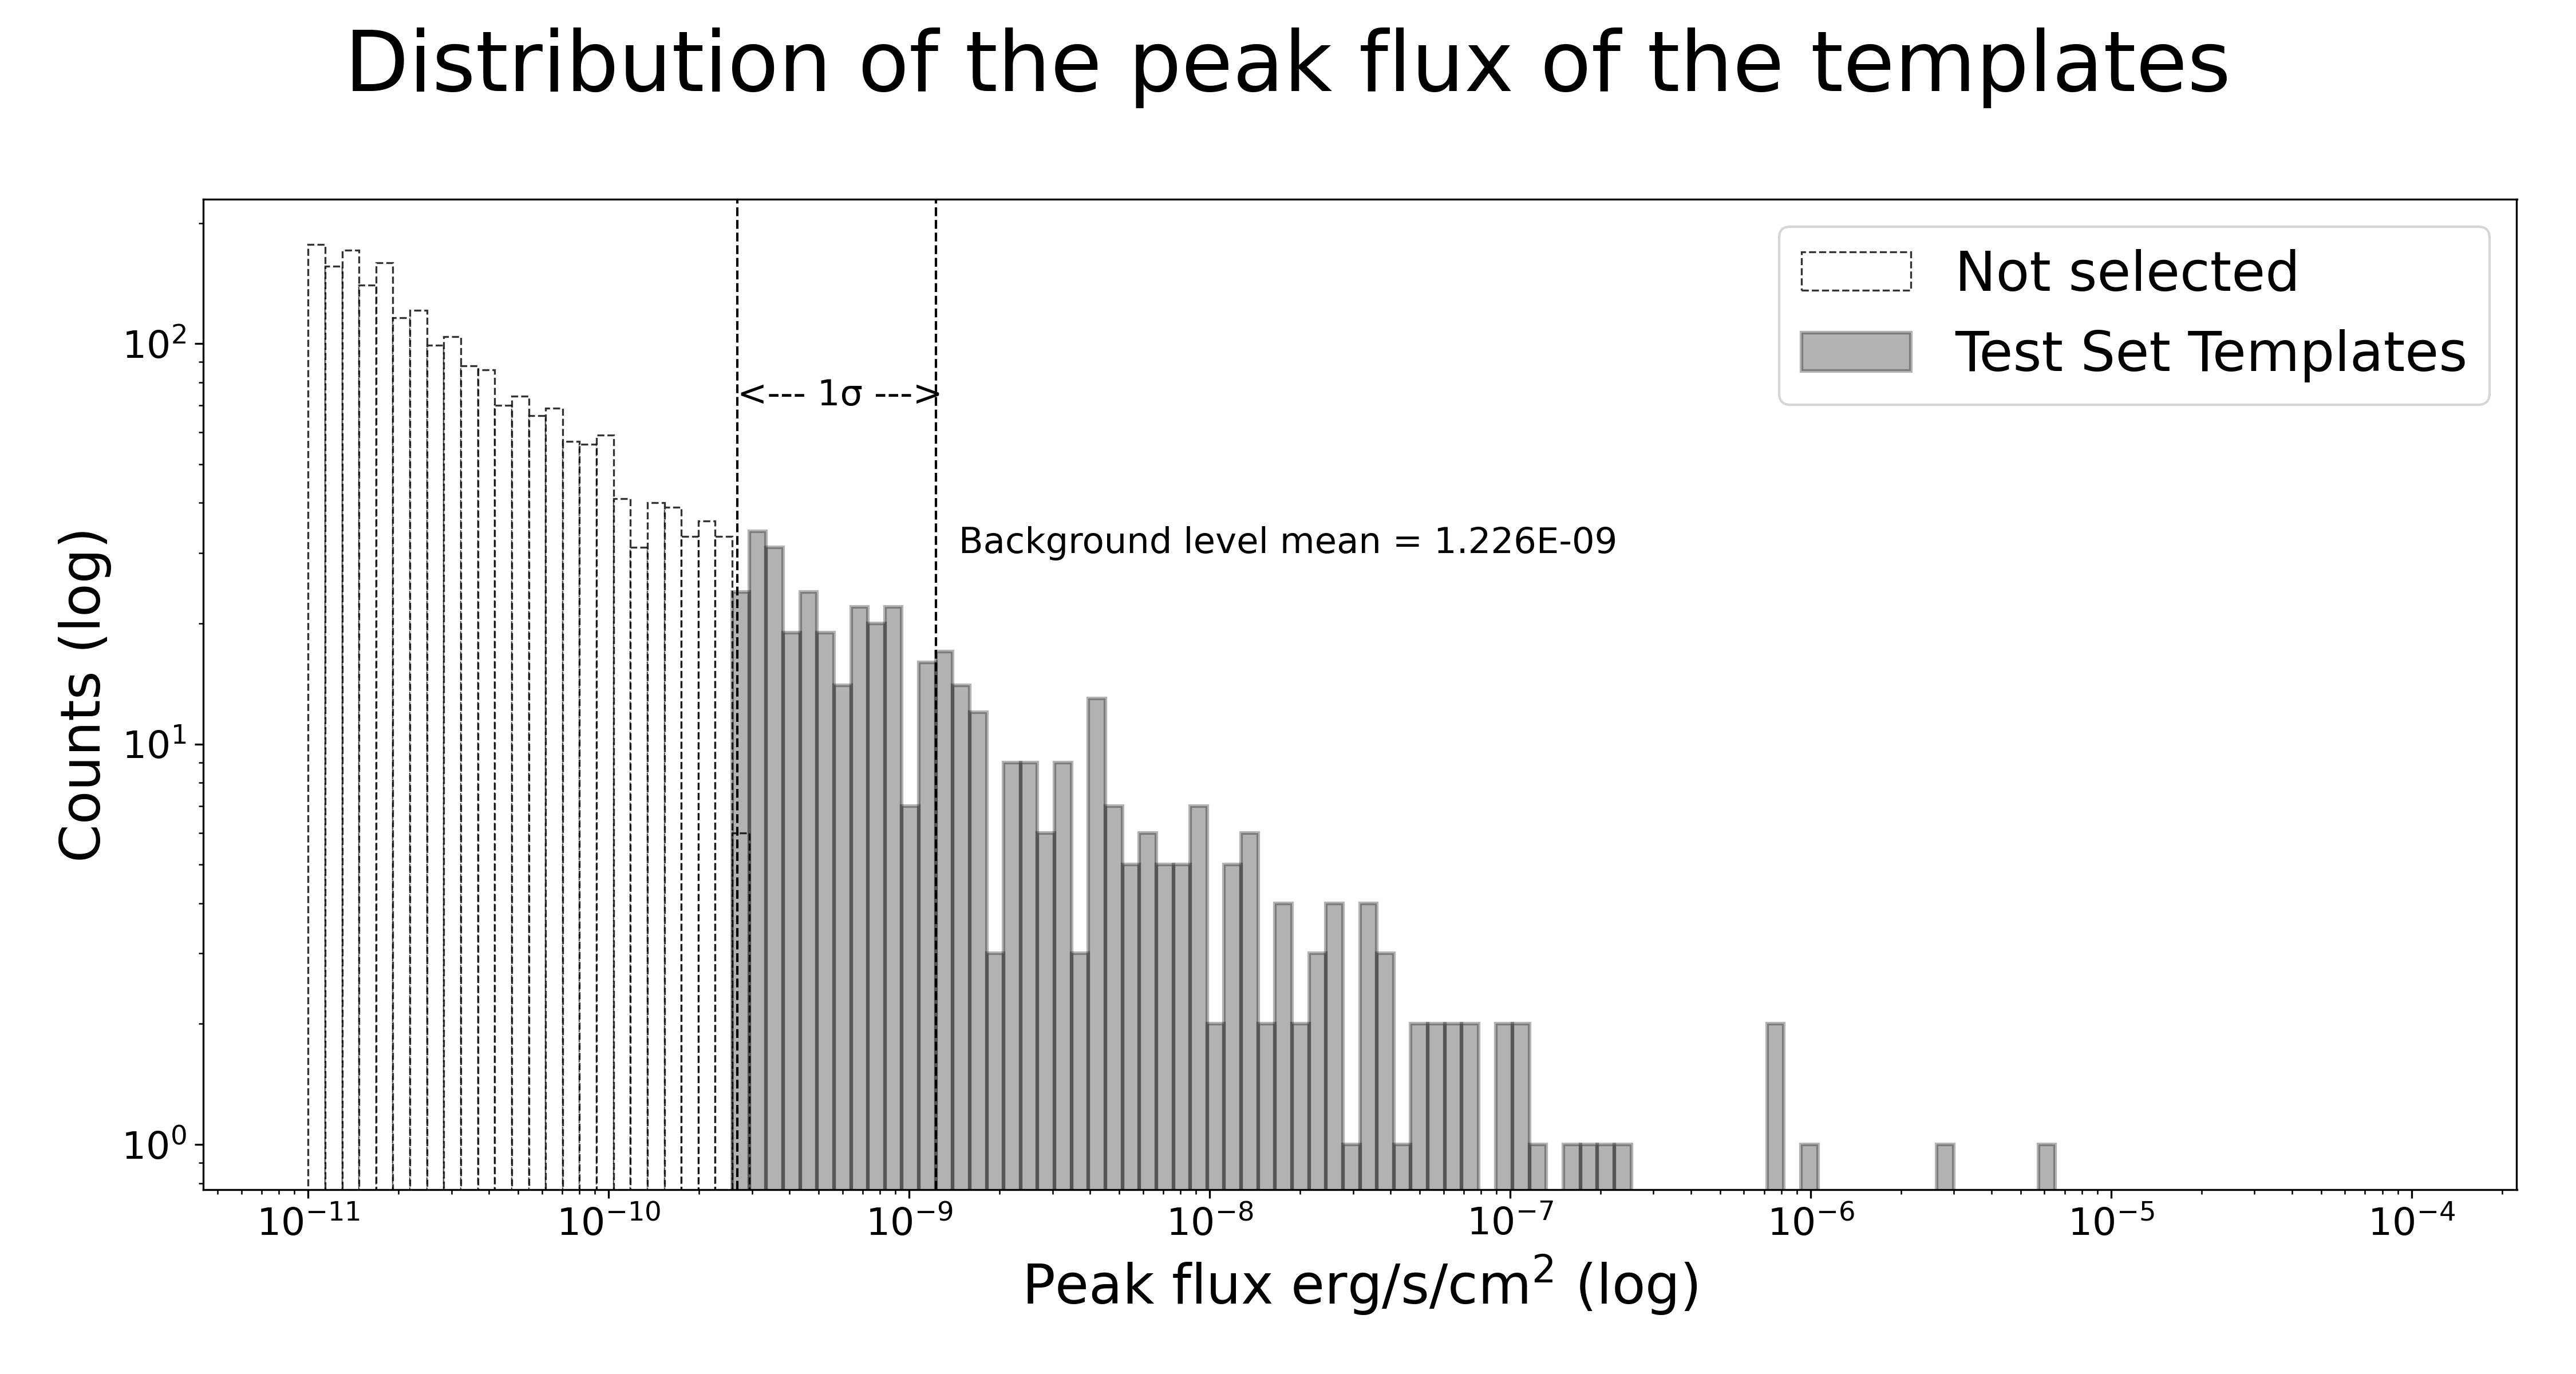
\includegraphics[width=1\textwidth]{figures/experiments/templates_max_flux_distributions.png}
\captionsetup{width=0.9\linewidth}
\caption{The distribution of the peak flux for each GRB template. The selected templates are 419, and their peak fluxes are within the $[2.6785e^{-10}, 1.1688e^{-04}]$. range.}
\label{f:exp-max-flux-distribution-E}
\end{figure}
The simulation time is limited to 500 seconds because we are interested in detecting the event as soon as possible. The trigger time that defines the start of the GRB event is fixed and equal to 250 seconds. The instrument response function (IRF) is the same used for generating the training set, which models the response of a sub-array configuration of 4 LST-1 telescopes located in the northern hemisphere site, observing for 5 hours at $40^{\circ}$ zenith angle.
As described in \autoref{ss:photometry-module}, the photons lists must be integrated in space, time, and energy to generate the multi-variate time series of flux measurements. The integration time is set to 5 seconds to evaluate the performances of the techniques in the short-exposure scenario and 1 second for the very short-exposure scenario. The integration process generates time series of 100 (short-exposure scenario) and 500 (very short-exposure scenario) flux measurements. Finally, as described in \autoref{ss:extractor}, the time series extractor module extracts sub-sequences from the generated time series. The length of the sub-sequences is fixed and set to 5 points, the same setting used to generate the data to train the auto-encoder. The stride parameter is set to 1 because the anomaly detection technique can use overlapping temporal bins, drastically reducing the time the model waits for data during the online inference. In contrast, the Li\&Ma technique must use temporal bins that are statistically independent. Finally, each sub-sequence is associated with a label. A sub-sequence is labeled as anomalous if at least one of its points exceeds the trigger time threshold that defines the start of the GRB event. For the short-exposure scenario (integration time = 5 seconds), the number of generated test samples is 40224, of which 20531 are labeled anomalous. For the very short-exposure scenario (integration time = 1 second), the number of test samples is 207824, of which 104331 are labeled anomalous. These configuration parameters are reported in \autoref{tab:test-set-fits} and \autoref{tab:test-set-ts}.

\begin{table}[]
\centering
\begin{tabular}{|l|l|}
\hline
\multicolumn{2}{|c|}{\textbf{Simulation parameters}} \\
\hline
trials          & 1                   \\ 
simtype         & grb                 \\ 
runid           &  [List of GRB templates] \\ 
scalefluxfactor & 1.0                 \\ 
caldb           & prod5-v0.1          \\ 
emin            & 0.04                \\ 
emax            & 1                   \\ 
irf             & North\_z40\_5h\_LST \\ 
offset          & $0.5\degree$        \\ 
roi             & $2.5\degree$        \\ 
tobs            & 500                 \\ \hline
\end{tabular}
\caption{The parameters used to customize the photon lists simulation for the test set generation. The list of templates (\textit{runid}) has been omitted due to limited space.}
\label{tab:test-set-fits}
\end{table}
\begin{table}[]
\centering
\begin{tabular}{|l|l|}
\hline
\multicolumn{2}{|c|}{\textbf{Test test (short-exposure)}} \\
\hline
integration\_time  & 5 \\ 
number\_of\_energy\_bins & 3 \\ 
normalize & True \\ 
sub\_window\_size & 5 \\ 
stride & 1 \\ 
Normal samples & 40224\\ 
Anomalous samples & 20531 \\  \hline
\end{tabular}
\quad
\begin{tabular}{|l|l|}
\hline
\multicolumn{2}{|c|}{\textbf{Train test (very short-exposure)}} \\
\hline
integration\_time  & 1 \\ 
number\_of\_energy\_bins & 3 \\ 
normalize & True \\ 
sub\_window\_size & 5 \\ 
stride & 1 \\ 
Normal samples & 207824\\ 
Anomalous samples & 104331 \\ \hline
\end{tabular}
\caption{The parameters used to configure the \textit{DataManager} class to extract sub-sequences with photometry and to generate the test set. The left panel shows the parameters of the short-exposure scenario, while the right panel shows the parameters of the very short-exposure scenario.}
\label{tab:test-set-ts}
\end{table}



\FloatBarrier
\section{P-value analysis results}
\label{s:p-values-results}
As outlined in \autoref{ss:p-values}, the p-value analysis is used to obtain the threshold $\tau$ to classify the samples as anomalies with a certain $\sigma$ level or, on the contrary, to associate with each anomaly score a statistical confidence level (of a positive classification). Four p-value analyses have been performed, one for each autoencoder model (convolutional and recurrent) in the short-exposure and very short-exposure settings. The models performed inferences on $1e^8$ background-only samples, and the distributions of the anomaly score (weighted mean squared error) have been computed. Then, the inverse cumulative of the distribution function was evaluated, and the mapping between the y-axis (p-values) and the x-axis (anomaly scores) was written on disk. 
\begin{figure}[!htb]
    \centering
    \begin{minipage}{0.5\textwidth}
        \centering
        \includesvg[width=\linewidth]{figures/experiments/p_val/model_1_ts.svg}
    \end{minipage}%
    \begin{minipage}{0.5\textwidth}
       \centering
       \includesvg[width=\linewidth]{figures/experiments/p_val/model_1_pvalues.svg}
    \end{minipage}
    \captionsetup{width=0.9\linewidth}
    \caption{TS distribution and p-values for the autoencoder with recurrent layers in the short-exposure scenario (integration time = 5 seconds).}
    \label{fig:ts-distribution-and-p-values-rnn-it-5}
\end{figure}

\begin{table}[!htb]
\centering
\begin{tabular}{|p{3cm}|p{3cm}|p{3cm}|p{3cm}|}
\hline
\multicolumn{4}{|c|}{p-values} \\
\hline
Threshold & p-value & $\pm$ error &  Sigma \\
\hline
0.003171 &  1.283972e-01 &  1.201785e-04 &  1.134 \\
0.003751 &  6.115264e-02 &  8.293861e-05 &  1.545 \\
0.004476 &  2.277199e-02 &  5.061155e-05 &  2.000 \\
0.005492 &  5.323285e-03 &  2.447028e-05 &  2.554 \\
0.006507 &  1.228234e-03 &  1.175411e-05 &  3.029 \\
0.007667 &  2.312711e-04 &  5.100465e-06 &  3.502 \\
0.009118 &  3.149606e-05 &  1.882250e-06 &  4.001 \\
0.010859 &  3.262092e-06 &  6.057553e-07 &  4.509 \\
0.013760 &  4.499438e-07 &  2.249719e-07 &  4.912 \\
0.013905 &  2.249719e-07 &  1.590791e-07 &  5.047 \\
\hline
\end{tabular}
\caption{An example of p-value analysis for the autoencoder with recurrent layers in the short-exposure scenario (integration time = 5 seconds). The table shows a subset of all the rows. Only the threshold values corresponding to predefined sigma levels are shown.}
\label{tab:p-value-table-rnn-itime-5}
\end{table}
The visualization tool of \cite{dipiano2022ctasagsci} has been used to compute the plots shown in \autoref{fig:ts-distribution-and-p-values-rnn-it-5}. The figure shows the p-value analysis results for the autoencoder with recurrent layers in the short-exposure scenario. The left panel  shows the test statistic distribution, and the right panel shows the corresponding p-values. \autoref{tab:p-value-table-rnn-itime-5} shows the actual values of the anomaly score - sigma level mapping. The number of rows of the table was limited to only certain levels of sigma. \autoref{s:appendix-a} lists the p-value analysis results for each model and analysis setting. 

 


\section{Comparison of the autoencoder architecures}
\label{s:architectures-comparison}
As described in Section \autoref{s:contribution}, the proposed anomaly detection technique utilizes an autoencoder model. Both convolutional and recurrent layer-based architectures for autoencoders have been examined. The chapter will compare their performances using standard machine learning metrics. The accuracy, precision, recall, and false positive rate metrics express the percentage of the time series correctly classified, what proportion of positive identifications was actually correct, what proportion of actual positives was identified correctly, and what proportion of the actual negative events were wrongly categorized as positive. While precision measures the probability of a sample classified as positive to be an actual positive sample, the false positive rate measures the ratio of false positives within the negative samples. The accuracy, precision, and recall values computed with different thresholds can help understand the evolution of trade-offs between the number of false positive and false negative classifications. \autoref{fig:rnn-metrics-itime-5} shows the accuracy, precision, and recall curves for the autoencoder model with recurrent layers in the short-exposure settings (integration time = 5). 
\begin{figure}[!htb]
    \centering
    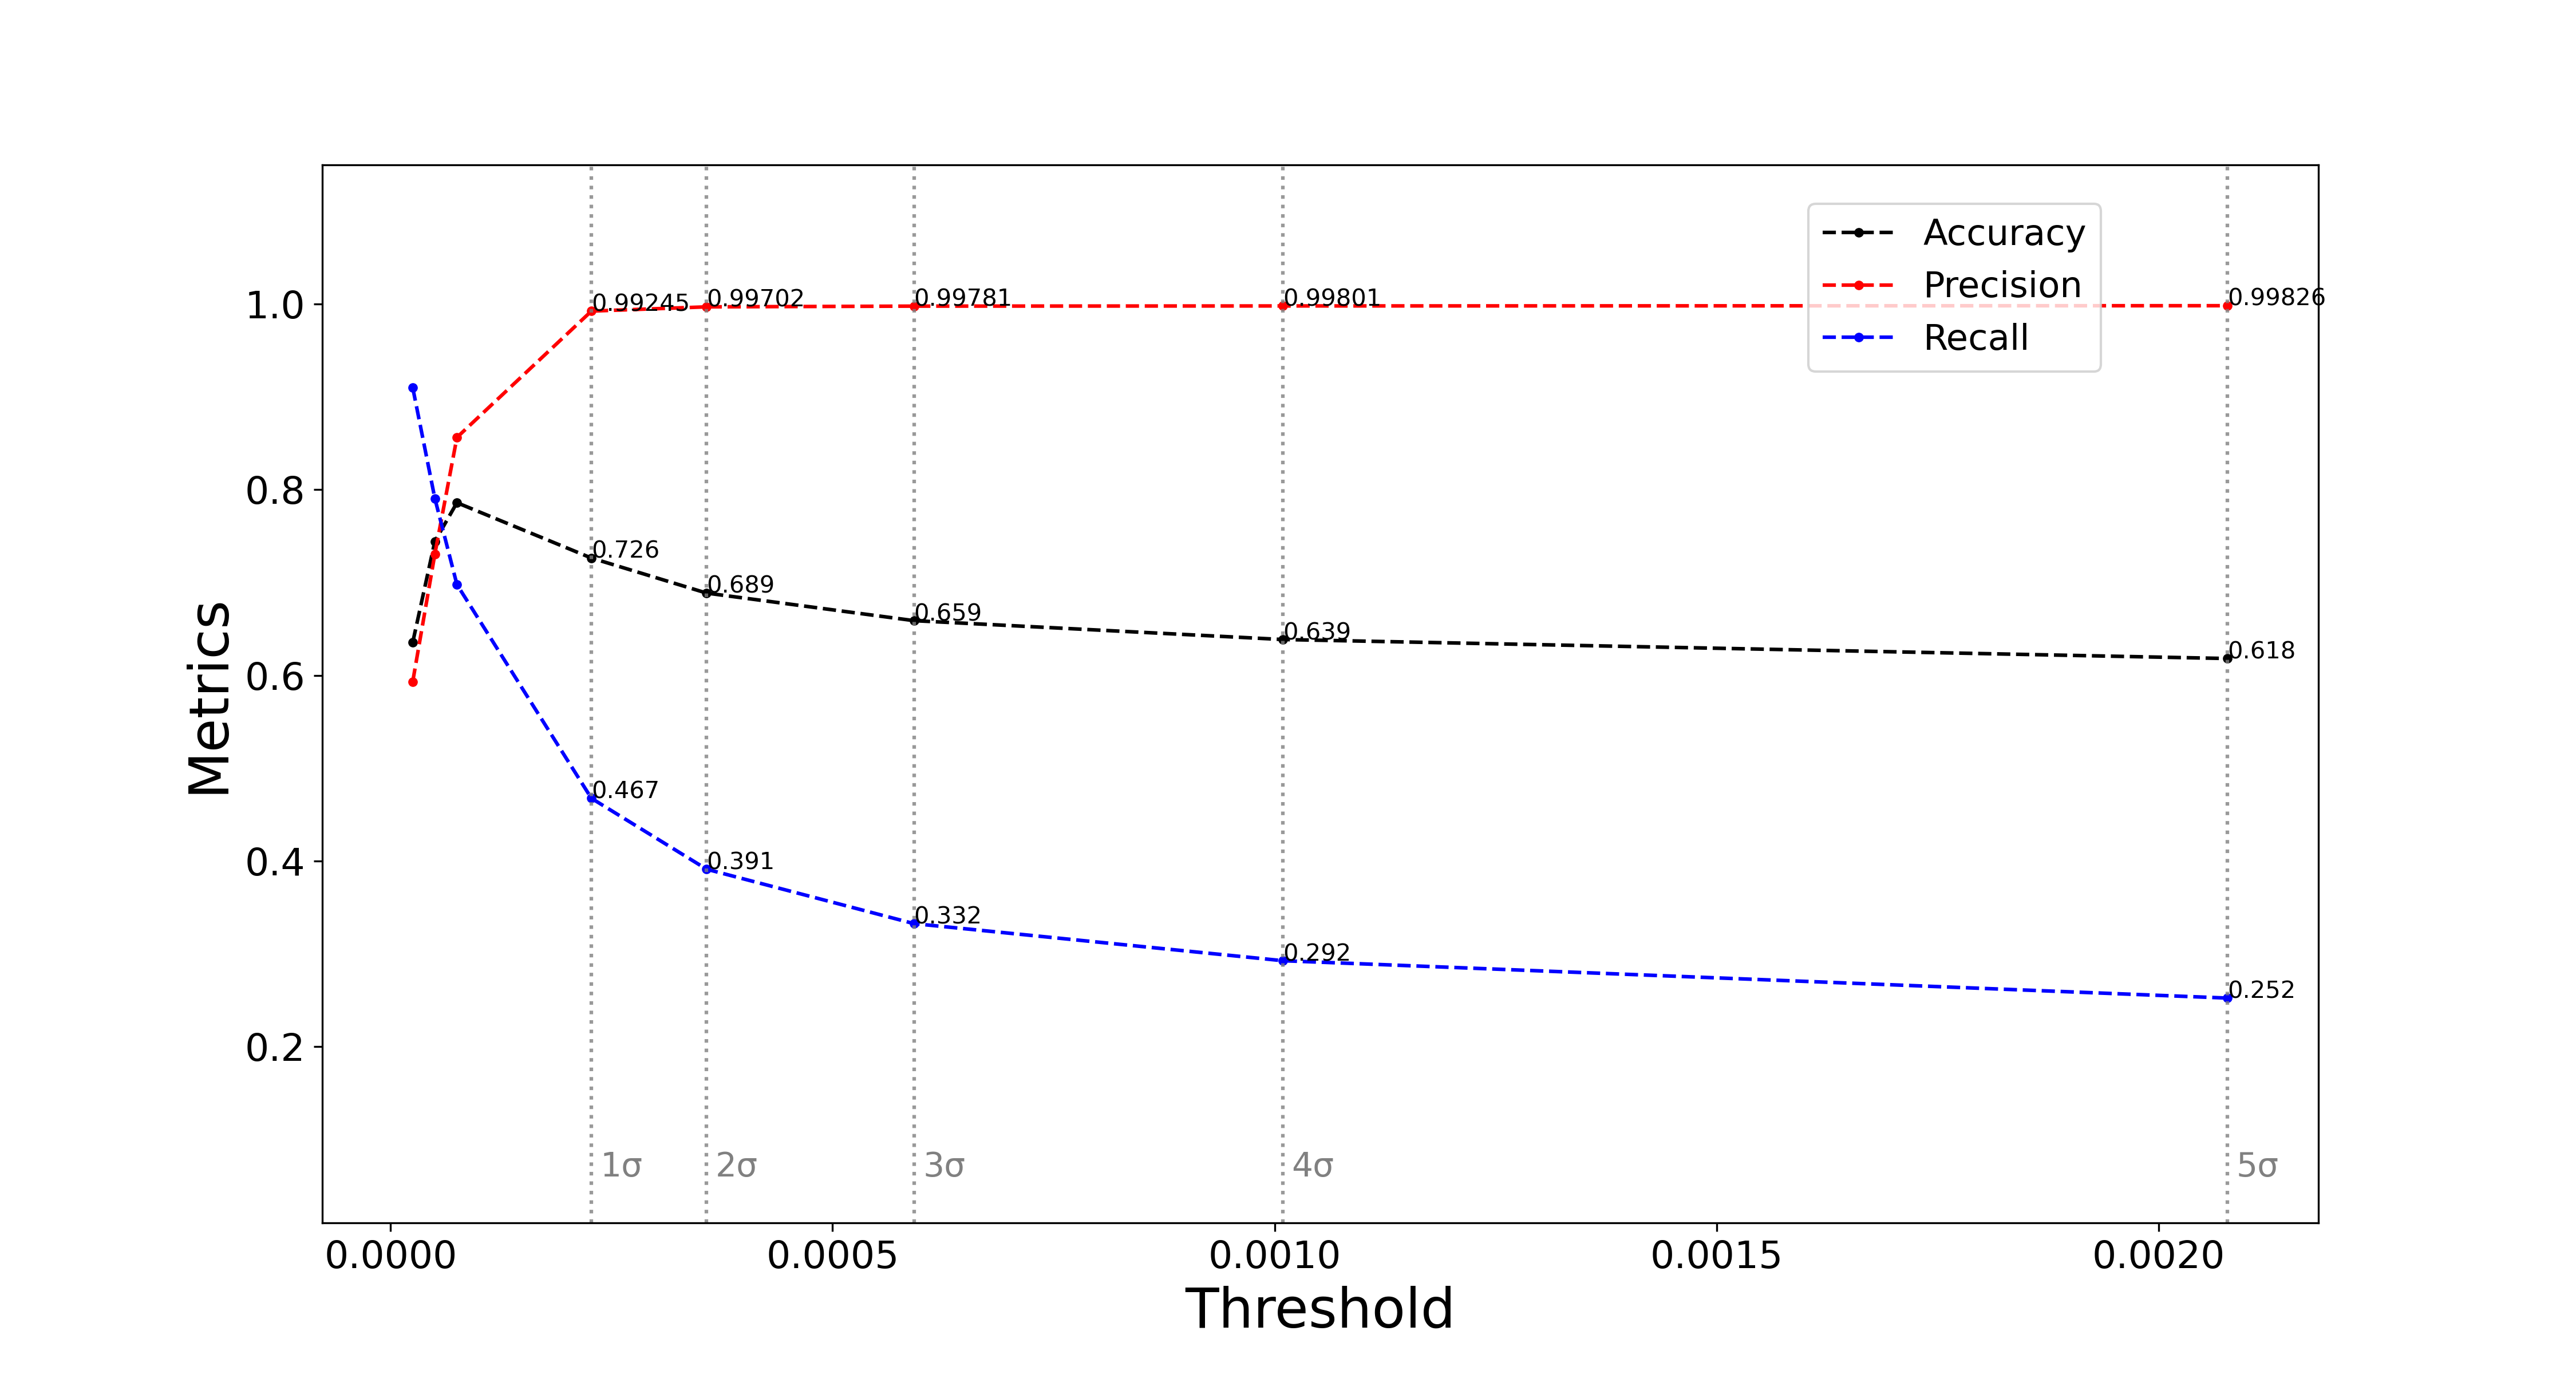
\includegraphics[width=\linewidth]{figures/experiments/metrics/rnn_metrics_test_set_all_itime_5.png}
    \captionsetup{width=0.9\linewidth}
    \caption{Accuracy, precision, and recall curves for the autoencoder model with recurrent layers in the short-exposure settings (integration time = 5).}
    \label{fig:rnn-metrics-itime-5}
\end{figure}
\autoref{tab:standard-metrics-itime-5} and \autoref{tab:standard-metrics-itime-1} show the actual values of accuracy, precision, recall, and false positive rate computed using the $5\sigma$ threshold, for both architectures and short-exposure settings. The autoencoder with recurrent layers obtained better accuracy and recall in both scenarios. At the same time, autoencoder with convolutional layers is less precise but has a better false positive rate. 
\begin{table}[!htb]
\centering
\begin{tabular}{|c|c|c|c|c|}
    \hline
    Model & Accuracy & Precision & Recall & False Positive Rate \\ 
    \hline
    RNN & $61.81\%$ & $99.83\%$ & $25.22\%$ & $0.17\%$ \\
    CNN & $59.96\%$ & $99.86\%$ & $21.58\%$ & $0.13\%$ \\
    \hline
    \end{tabular}
\caption{Standard metrics in the short-exposure settings (integration time = 5), using the $5\sigma$ threshold. The number of test samples is 40224, of which 20531 are anomalous.}
\label{tab:standard-metrics-itime-5}
\vspace{1cm}
\centering
\begin{tabular}{|c|c|c|c|c|}
    \hline
    Model & Accuracy & Precision & Recall & False Positive Rate \\ 
    \hline
    RNN & $57.05\%$ & $99.97\%$ & $14.46\%$ & $0.033\%$ \\
    CNN & $55.58\%$ & $99.98\%$ & $11.52\%$ & $0.016\%$ \\
    \hline
\end{tabular}
\caption{Standard metrics in the very short-exposure settings (integration time = 1), using the $5\sigma$ threshold. The number of test samples is 207824, of which 104331 are anomalous.}
\label{tab:standard-metrics-itime-1}
\end{table}
\autoref{s:appendix-b} presents the same metrics for each model and analysis setting. 


\FloatBarrier
\section{Evaluation of the proposed technique against Li\&Ma}
\label{s:ad-vs-lima}
The performances of the proposed anomaly detection method have been evaluated against Li\&Ma, the standard technique used to address the source detection problem in the ground-based gamma-ray astronomy field.
\FloatBarrier
\subsection{Key performance indicators}
The first key performance indicator is the cumulative number of $5\sigma$ detections. This metric evaluates the robustness of the techniques. As outlined in \autoref{s:Experiment-Data}, the data set for testing is composed of 419 simulated GRB events. The number of $5\sigma$ detections is evaluated for each time bin whose time span depends on the integration time and the length of the sub-sequences. This number is cumulated for the following time bins. 

For the reasons stated in the previous section, evaluating how fast the technique is to issue $5\sigma$ detections is crucial. Hence the second key performance indicator represents the average time to perform detections. This metric is called \textit{Detection Delay} (DD) and is evaluated as follows. For each time bin, the number of seconds between the start of the GRB event ($t_{grb}=250s$) and the detection time, is computed. This delay ($d_{tb}$) is the same for each detection performed in a time bin. For example, if the autoencoder model performs a detection in time bin $[230-255]$, the delay ($d_{[230-255]}$) is equal to 5 seconds ($255-250$). The delay is computed for each time bin. Then, a weighted average is evaluated, considering the number of the detections in common to the two techniques within the time bins, from $[245-250]$ to $tb_{max}$. Considering the short-exposure scenario, the detection delay (DD) is defined as:
$$
    DD = \frac{1}{tcd} \sum_{tb=[245-250]}^{tb_{max}} w_{tb}*d_{tb}
$$
Where $tcd$ is the total number of detections in common to the two methods, $w_{tb}$ represents the number of detections made in a particular time bin, and $d_i$ is the delay expressed as the difference between $tb$ and the time bin of the start of the GRB event ($t_{grb}=250s$). 

\FloatBarrier
\subsection{Serendipitous discovery results}
\label{s:Serendipitous-Discoveries-Results}
In the serendipitous discovery scenario, while the telescopes are observing a particular target, an unexpected event appears in the field of view. The issue is that we don't know in which region the GRB event will appear. This study assumes a blind-search analysis applied to the whole field of view to determine the aperture photometry regions. In particular, it is assumed that the blind-search analysis will always find the region that contains the GRB event in its center and will take a fixed time of 10 seconds to complete.

\FloatBarrier
\subsubsection{Short-exposure scenario}
\label{s:Serendipitous-Discoveries-Results-Short-Term}
\autoref{f:serendipitous-discoveries-itime-5} shows the cumulative number of detections performed by the anomaly detection and Li\&Ma techniques for each temporal bin in the short-exposure scenario (integration time = 5 seconds). The x-axis holds each temporal bin. The y-axis holds the cumulative number of detections among all the GRB events.  The vertical dashed line corresponds to the start of the GRB event. The grey area represents the application of the blind-search algorithm, so even if the series start at bin $[225-250]$, only the points outside the grey area must be considered.
\begin{figure}[!ht]
\centering
\includesvg[width=1\textwidth]{figures/experiments/results/serendipitous_discoveries_time_5.svg}
\captionsetup{width=0.9\linewidth}
\caption{The cumulative number of detections of anomaly detection and Li\&Ma techniques for each temporal bin in the short-exposure scenario (integration time = 5 seconds). The x-axis holds each temporal bin. The y-axis holds the cumulative number of detections among all the GRB events. The vertical dashed line corresponds to the start of the GRB event. The grey area represents the application of the blind-search algorithm.}
\label{f:serendipitous-discoveries-itime-5}
\end{figure}
The figure shows the robustness of the Li\&Ma technique, detecting at the end of the observation more GRBs than the anomaly detection technique. However, we are interested in the first part of the observation since detections must be performed as soon as possible. The anomaly detection technique can be applied after each $T=5$ seconds of new data. In contrast, Li\&Ma is limited by statistical independence assumption and can be applied only for temporal bins that do not overlap. To quantify how faster the anomaly detection technique is with respect to Li\&Ma, \autoref{tab:dd-itime-5-common} shows the DD metric. The first temporal bin considered in the table starts when the blind-search algorithm ends. The next temporal bins are the ones in which Li\&Ma was applied. To be fairer in the comparison against Li\&Ma, \autoref{tab:dd-itime-5-common} reports the same metrics but considers only the same detections performed by both anomaly detection and Li\&Ma techniques. The tables prove the ability of the anomaly detection technique to perform faster detections with respect to Li\&Ma.


 
\begin{table}[!ht]
\centering
\begin{tabular}{|c|rl|rl|rl|} 
\hline
\multicolumn{7}{|c|}{\textbf{Detection delay} (common detections)} \\ 
\hline
\multicolumn{1}{|c|}{Temporal bins} & \multicolumn{2}{c|}{CNN} & \multicolumn{2}{c|}{RNN} & \multicolumn{2}{c|}{Li\&Ma} \\ 
\hline
250-275 &  6.86 &  $\pm$5.41 &  6.37 &  $\pm$5.57 & 15.00 &  $\pm$0 \\
275-300 & 10.78 &  $\pm$9.25 & 12.04 & $\pm$11.56 & 21.28 & $\pm$10.87 \\
300-325 & 14.28 & $\pm$13.69 & 15.98 & $\pm$15.58 & 24.87 & $\pm$14.6 \\
325-350 & 17.02 & $\pm$17.31 & 18.87 & $\pm$18.75 & 27.64 & $\pm$17.9 \\
350-375 & 18.98 & $\pm$19.88 & 21.31 & $\pm$21.79 & 29.59 & $\pm$20.25 \\
\hline
\end{tabular}
\caption{Detection delay (in seconds) for serendipitous discoveries in the short-exposure scenario (integration time = 5 seconds) with common detections.}
\label{tab:dd-itime-5-common}
\end{table}






\FloatBarrier
\subsubsection{Very short-exposure scenario}
\label{s:Serendipitous-Discoveries-Results-Very-Short-Term}
The same metrics are evaluated again in the very short-exposure scenario, with an integration time equal to 1 second. In this scenario, the number of photon counts is further reduced, often exceeding the lower bounds of the Li\&Ma technique (equal to 10 photon counts from the on and off regions), limiting its applicability. In contrast, it reduces from 5 to 1 second the time the anomaly detection technique needs to wait for new data since a new flux data measurement is available each second, and a new sub-sequence is ready for analysis. This time is also reduced for Li\&Ma, from 25 to 5 seconds. 
\autoref{f:serendipitous-discoveries-itime-1} shows that the number of detections performed by the anomaly detection technique with recurrent layers is always greater than Li\&Ma's one, proving greater robustness in this extreme scenario. As said before, the Li\&Ma is not always applicable due to its limitation of requiring at least 10 photon counts. The reduced number of photon counts also negatively affects the performance of the anomaly detection technique. It's also worth noticing that the anomaly detection technique with convolutional layers has better performance with respect to Li\&Ma from the beginning of the observation until the $[295-300]$ temporal bin. Concerning the detection delay, \autoref{tab:dd-itime-5-common} and \autoref{tab:dd-itime-1-common} show that the anomaly detection technique is faster with respect to Li\&Ma, also in the very short-exposure scenario.

\begin{figure}[!ht]
\centering
\includesvg[width=1\textwidth]{figures/experiments/results/serendipitous_discoveries_time_1.svg}
\captionsetup{width=0.9\linewidth}
\caption{The cumulative number of detections of anomaly detection and Li\&Ma techniques for each temporal bin in the very short-exposure scenario (integration time = 1 seconds). The x-axis holds each temporal bin. The y-axis holds the cumulative number of detections among all the GRB events. The vertical dashed line corresponds to the start of the GRB event. The grey area represents the application of the blind-search algorithm.}
\label{f:serendipitous-discoveries-itime-1}
\end{figure}

 
\begin{table}[!ht]
\centering
\begin{tabular}{|c|cc|cc|cc|} 
\hline
\multicolumn{7}{|c|}{\textbf{Detection delay} (common detections)} \\ 
\hline
\multicolumn{1}{|c|}{Temporal bins} & \multicolumn{2}{c|}{RNN} & \multicolumn{2}{c|}{CNN} & \multicolumn{2}{c|}{Li\&Ma} \\ 
\hline
280-285 & 10.11 &  $\pm$7.46 & 11.04 &  $\pm$7.54  & 11.57 &  $\pm$8.46\\
305-310 & 13.77 & $\pm$11.69 & 13.86 &  $\pm$9.86 & 17.01 & $\pm$13.86\\
330-335 & 15.39 & $\pm$13.56 & 15.93 & $\pm$12.46 & 19.8 & $\pm$16.39 \\
355-360 & 17.24 & $\pm$16.41 & 17.14 & $\pm$13.95 & 22.31 & $\pm$19.48 \\
380-385 & 18.95 & $\pm$19.27 & 18.65 & $\pm$17.28 & 24.35 &$\pm$22.23 \\
\hline
\end{tabular}
\caption{Detection delay (in seconds) for serendipitous discoveries in the very short-exposure scenario (integration time = 1 seconds) with common detections.}
\label{tab:dd-itime-1-common}
\end{table}




\FloatBarrier
\subsection{Follow-up observation results}
\label{s:Follow-Up-Observation-Results}
In the follow-up observation scenario, the facility receives a scientific alert and adjusts the pointing of its telescope to a new sky region to detect the event. This study considers the variable delay between the event's start and the taking of the first photon counts, which depends on the time to receive the scientific alert and the time the telescopes take to change the pointing. Four delay values are considered (25, 50, 75, and 100 seconds). If the localization error of the source provided by the scientific alert is too large, for example in the case of gravitational-waves alerts discussed in \autoref{ss:scientific-use-cases-and-assumptions}, a blind-search algorithm is assumed to start at soon as the telescopes take data. As in the serendipitous discovery scenario, the blind-search algorithm is always assumed to find the right region in a fixed time of 10 seconds. The cumulative detection plot is repeated four times for clarity in different sub-plots. Each subplot shows a vertical line representing the follow-up observation's start. The next vertical line, represents the time the techniques need to wait to gather enough data to make the first inference. 

\FloatBarrier
\subsubsection{Short-exposure scenario}
\label{s:Follow-Up-Observation-Results-Short-Term}
Due to the delay that postpones the observation, the evolution of the GRB event cannot be observed from the beginning. The luminosity of a GRB event tends to decrease over time, increasing the difficulty of detection. \autoref{fig:follow-up-itime-5} shows the superiority of the Li\&Ma technique in the short-exposure scenario. The cumulative number of detections is greater for Li\&Ma for every temporal bin, and as a consequence, its detection delay, shown in \autoref{tab:dd-follow-up-itime-5-common}, is also better.


\begin{figure}[!ht]
\centering
\includesvg[width=1.1\textwidth]{figures/experiments/results/follow_up_itime_5.svg}
\captionsetup{width=1\linewidth}
\caption{The cumulative number of detections of anomaly detection and Li\&Ma techniques for each temporal bin in the short-exposure scenario (integration time = 5 seconds). The x-axis holds each temporal bin. The y-axis holds the cumulative number of detections among all the GRB events. The vertical dashed line corresponds to the start of the GRB event.}
\label{fig:follow-up-itime-5}
\end{figure}


\begin{table}[!ht]
\centering
\begin{tabular}{|c|cc|cc|cc|} 
\hline
\multicolumn{7}{|c|}{\textbf{Detection delay} (common detection)} \\ 
\hline
\multicolumn{1}{|c|}{Temporal bins} & \multicolumn{2}{c|}{RNN} & \multicolumn{2}{c|}{CNN} & \multicolumn{2}{c|}{Li\&Ma} \\ 
\hline
275-300 &  25    & $\pm$0 & 25 &  $\pm$0 & 25 &  $\pm$0  \\
300-325 & 35.94 & $\pm$7.79 & 33.54 &  $\pm$9.26 & 28.68 &  $\pm$8.89 \\
325-350 & 41.5  & $\pm$13.5 & 38.37 & $\pm$13.59 & 32.01 & $\pm$13.83 \\
350-375 & 45    & $\pm$17.08 & 43.04 & $\pm$18.42 & 34.32 & $\pm$16.95  \\
375-400 & 48.71 & $\pm$21.82 & 48.25 & $\pm$24.32 & 36.71 & $\pm$20.75  \\
\hline
\end{tabular}
\caption{Detection delay (in seconds) for follow-up observations in the short-exposure scenario (integration time = 5 seconds) for common detection.}
\label{tab:dd-follow-up-itime-5-common}
\end{table}
 

\FloatBarrier
\subsubsection{Very short-exposure scenario}
\label{s:Follow-Up-Observation-Results-Very-Short-Term}
The same metrics were evaluated in a short-exposure scenario with 1 second integration time. The same considerations for the serendipitous discovery use case can be made here—the very short-exposure scenario leads to fewer photon counts but faster data availability. The reduced photon counts negatively affected the performance of the anomaly detection and Li\&Ma techniques. The anomaly detection technique based on the autoencoder with recurrent layers showed greater robustness than Li\&Ma and was faster in detecting anomalies. \autoref{fig:follow-up-itime-1} shows the cumulative number of detections. Also, in this case, the anomaly detection technique with convolutional layers has better performance with respect to Li\&Ma from the beginning of the observation until the $295-300$ temporal bin. The detection delay, shown in \autoref{tab:dd-follow-up-itime-1-common}, is always lower for anomaly detection with recurrent and convolutional layers, despite the CNN-Li\&Ma performance-flip within bin $295-300$.



\begin{figure}[!ht]
\centering
\includesvg[width=1.1\textwidth]{figures/experiments/results/follow_up_itime_1.svg}
\captionsetup{width=1\linewidth}
\caption{The cumulative number of detections of anomaly detection and Li\&Ma techniques for each temporal bin in the very short-exposure scenario (integration time = 1 seconds). The x-axis holds each temporal bin. The y-axis holds the cumulative number of detections among all the GRB events. The vertical dashed line corresponds to the start of the GRB event.}
\label{fig:follow-up-itime-1}
\end{figure}


\begin{table}[!ht]
\centering
\begin{tabular}{|c|cc|cc|cc|} 
\hline
\multicolumn{7}{|c|}{\textbf{Detection delay} (common detection)} \\ 
\hline
\multicolumn{1}{|c|}{Temporal bins} & \multicolumn{2}{c|}{RNN} & \multicolumn{2}{c|}{CNN} & \multicolumn{2}{c|}{Li\&Ma} \\ 
\hline
260-265 & 5 &  $\pm$0 & 5 &  $\pm$0 & 5 &  $\pm$0 \\
290-295&15.78&$\pm$7.71&16.74&$\pm$6.82&14.65&$\pm$7.82\\
315-320&18.74&$\pm$11.07&19.13&$\pm$11.26&19.62&$\pm$12.74\\
340-345&20.46&$\pm$13.2&20.31&$\pm$13.14&22.49&$\pm$15.72\\
365-370&22.86&$\pm$16.96&20.82&$\pm$13.83&24.78&$\pm$18.48\\
\hline
\end{tabular}
\caption{Detection delay (in seconds) for follow-up observations in very the short-exposure scenario (integration time = 1 second) for common detections.}
\label{tab:dd-follow-up-itime-1-common}
\end{table}

\FloatBarrier
\section{Summary}
This chapter presented the results of p-value analyses and performance benchmarks. It reintroduced the scientific use cases and the assumptions made in these scenarios and described the process of test set generation. The results of the p-value analysis were shown, followed by a comparison between the two investigated autoencoder architectures. The performance of the proposed anomaly detection was compared against Li\&Ma, using key performance indicators, with results presented for both serendipitous discoveries and follow-up observation scenarios in the short-exposure and very short-exposure.